% ============================================================================
% Prakshep: IEEE Conference Paper
% Digital Twin & RL Trajectory Optimization Engine for ISRO Launch Vehicles
% ============================================================================
\documentclass[conference]{IEEEtran}

% ── Packages ────────────────────────────────────────────────────────────────
\usepackage{cite}
\usepackage{amsmath,amssymb,amsfonts}
\usepackage{graphicx}
\usepackage{textcomp}
\usepackage{xcolor}
\usepackage{hyperref}
\usepackage[ruled,vlined,linesnumbered]{algorithm2e}
\usepackage{listings}
\usepackage{booktabs}
\usepackage{multirow}
\usepackage{subcaption}

% ── Hyperref Configuration ──────────────────────────────────────────────────
\hypersetup{
    colorlinks=true,
    linkcolor=blue,
    citecolor=blue,
    urlcolor=blue,
    bookmarksnumbered=true,
}

% ── Listings Configuration ──────────────────────────────────────────────────
\lstset{
    basicstyle=\ttfamily\footnotesize,
    keywordstyle=\color{blue},
    commentstyle=\color{green!60!black},
    stringstyle=\color{red!70!black},
    numbers=left,
    numberstyle=\tiny\color{gray},
    frame=single,
    breaklines=true,
    captionpos=b,
}

% ── Custom Commands ─────────────────────────────────────────────────────────
\newcommand{\vect}[1]{\boldsymbol{#1}}
\newcommand{\mat}[1]{\mathbf{#1}}
\def\BibTeX{{\rm B\kern-.05em{\sc i\kern-.025em b}\kern-.08em
    T\kern-.1667em\lower.7ex\hbox{E}\kern-.125emX}}

% ============================================================================
\begin{document}

\title{Prakshep: A Digital Twin and Reinforcement Learning Trajectory Optimization Engine for ISRO Launch Vehicles}

\author{
    \IEEEauthorblockN{Aditya Sachin Khamitkar}
    \IEEEauthorblockA{
        \textit{School of Computing and Artificial Intelligence}\\
        \textit{VIT Bhopal University}\\
        Bhopal, India\\
        adityakhamitakr2022@vitbhopal.ac.in
    }
}

\maketitle

\IEEEpeerreviewmaketitle

% ============================================================================
% ABSTRACT
% ============================================================================
\begin{abstract}
This paper presents \textit{Prakshep}, a comprehensive open-source digital twin and trajectory optimization engine designed for the simulation of Indian Space Research Organisation (ISRO) launch vehicles, including the PSLV-XL, GSLV Mk~II, and LVM3. The system integrates a high-fidelity C++ six-degree-of-freedom (6-DOF) physics engine---incorporating Runge-Kutta 4th order numerical integration, J2 gravitational perturbation modeling, and the US Standard Atmosphere 1976---with a Python-based reinforcement learning (RL) layer that trains Proximal Policy Optimization (PPO) and Soft Actor-Critic (SAC) agents for autonomous guidance, navigation, and control (GNC). A novel continuous learning pipeline enables RL agents to train from user-defined mission scenarios in real time. An LSTM-based anomaly detection module provides both pre-launch failure mode prediction and in-flight structural integrity monitoring, supporting autonomous flight termination logic. The system delivers real-time synthetic telemetry at 60~Hz through a FastAPI WebSocket server to a Next.js frontend featuring AAA-quality WebGPU rendering with physically-based materials, volumetric atmospheric scattering, and CesiumJS-powered ground-track visualization. \textit{Prakshep} demonstrates that a fully integrated digital twin---combining physics simulation, machine learning, and cinematic visualization---can be developed as an accessible, zero-cost research platform for launch vehicle trajectory analysis.
\end{abstract}

\begin{IEEEkeywords}
Digital Twin, Reinforcement Learning, Trajectory Optimization, ISRO, Launch Vehicle Simulation, 6-DOF Dynamics
\end{IEEEkeywords}

% ============================================================================
% I. INTRODUCTION
% ============================================================================
\section{Introduction}

India's space program has undergone a remarkable transformation over the past two decades, establishing itself as one of the world's most cost-effective and reliable launch service providers. From the record-breaking deployment of 104 satellites on a single PSLV mission in 2017 to the successful Chandrayaan-3 lunar landing in 2023, ISRO has demonstrated engineering excellence that demands equally sophisticated simulation and analysis tools. As mission profiles grow in complexity---encompassing reusable launch vehicles, human spaceflight under the Gaganyaan program, and interplanetary missions---the need for high-fidelity, accessible digital twin platforms becomes paramount.

Existing launch vehicle simulators fall broadly into two categories: proprietary, export-controlled systems developed by aerospace organizations such as NASA's POST (Program to Optimize Simulated Trajectories)~\cite{brauer1977post} and AGI's STK, which are prohibitively expensive and restricted; and academic tools that, while accessible, typically lack integration between physics simulation, machine learning, and real-time visualization. The aerospace simulation landscape thus presents a significant gap: no open-source platform currently provides a unified framework that combines high-fidelity 6-DOF dynamics, reinforcement-learning-based GNC optimization, and production-quality 3D rendering within a single, deployable system.

\textit{Prakshep} (Sanskrit: \textit{trajectory} or \textit{launch}) addresses this gap with four principal contributions:

\begin{enumerate}
    \item A \textbf{C++ 6-DOF physics engine} implementing RK4 integration, J2 gravitational perturbation, the US Standard Atmosphere 1976, Mach-dependent aerodynamics, and multi-stage propulsion models calibrated against publicly available ISRO launch vehicle specifications.
    \item A \textbf{reinforcement learning framework} built on Stable Baselines3~\cite{raffin2021stable} that trains PPO and SAC agents for continuous thrust vector control, with a novel continuous learning pipeline that ingests user-defined mission scenarios.
    \item An \textbf{LSTM-based anomaly detection system} capable of identifying pre-launch failure modes (cryogenic valve anomalies, LOX boil-off, IMU drift) and in-flight structural integrity violations.
    \item A \textbf{full-stack real-time visualization platform} delivering 60~Hz telemetry via FastAPI WebSockets to a Next.js frontend featuring WebGPU-accelerated PBR rendering and CesiumJS ground-track mapping.
\end{enumerate}

The remainder of this paper is organized as follows: Section~II describes the overall system architecture; Section~III presents the mathematical models underpinning the physics engine; Section~IV details the reinforcement learning methodology; Section~V discusses implementation considerations; Section~VI documents the supported launch vehicle configurations; Section~VII presents preliminary results; and Section~VIII concludes with future work directions.

% ============================================================================
% II. SYSTEM ARCHITECTURE
% ============================================================================
\section{System Architecture}

\textit{Prakshep} adopts a modular, layered architecture designed to separate concerns across four principal subsystems: the physics core, the machine learning layer, the backend telemetry server, and the frontend visualization platform. Fig.~\ref{fig:architecture} illustrates the overall data flow.

\begin{figure}[htbp]
    \centering
    \fbox{\parbox{0.9\linewidth}{\centering\vspace{1.5cm} System Architecture Diagram \\ (C++ Engine $\rightarrow$ pybind11 $\rightarrow$ Python ML $\rightarrow$ FastAPI $\rightarrow$ Next.js) \vspace{1.5cm}}}
    \caption{High-level system architecture of \textit{Prakshep} showing the data flow from the C++ physics engine through the Python ML layer and FastAPI backend to the Next.js frontend.}
    \label{fig:architecture}
\end{figure}

\subsection{C++ Physics Core}
The physics engine is implemented in C++17 for maximum computational performance. It encapsulates the 6-DOF equations of motion, the RK4 numerical integrator, the J2-perturbed gravity model, the US Standard Atmosphere 1976, Mach-dependent aerodynamic drag computation, and multi-stage propulsion models. The engine is designed as a stateless step function: given a state vector $\vect{y} \in \mathbb{R}^{14}$ and a control input vector $\vect{u} \in \mathbb{R}^{3}$ (pitch gimbal, yaw gimbal, throttle), it returns the next state vector after one integration step. This stateless design enables deterministic replay and parallelized RL training.

\subsection{pybind11 Bridge}
The C++ engine is exposed to Python via pybind11~\cite{jakob2017pybind11}, which provides near-zero-overhead bindings and supports NumPy-compatible buffer protocols. The binding layer marshals the 14-element state vector and 3-element control vector as contiguous NumPy arrays, avoiding serialization overhead. A \texttt{PrakshepSim} Python class wraps the C++ simulator, providing \texttt{reset()}, \texttt{step(action)}, and \texttt{get\_state()} methods compatible with the OpenAI Gym~\cite{brockman2016openai} interface.

\subsection{Python ML/RL Layer}
The machine learning layer comprises two subsystems: (a) a Gymnasium-compatible reinforcement learning environment that wraps the C++ physics engine, enabling training of PPO and SAC agents via Stable Baselines3; and (b) an LSTM-based anomaly detection module trained on synthetic failure-mode telemetry. Both subsystems operate within the same Python process, allowing the RL agent and anomaly detector to share the simulation state without inter-process communication overhead.

\subsection{FastAPI WebSocket Server}
The backend server, built on FastAPI~\cite{ramirez2018fastapi}, manages simulation lifecycle, streams telemetry, and persists flight data. A dedicated WebSocket endpoint pushes the full state vector at 60~Hz to connected frontend clients. Telemetry is simultaneously written to Apache Parquet files for post-flight analysis and optionally to a MinIO object store for long-term retention. RESTful endpoints expose simulation configuration, launch vehicle selection, and RL agent management.

\subsection{Next.js Frontend}
The frontend is a Next.js 14 application featuring three primary views: (a) a mission control room UI built with React and Shadcn/ui components, displaying real-time gauges, strip charts, and event timelines styled after ISRO's Mission Control Centre; (b) a WebGPU-accelerated 3D viewport rendered via React Three Fiber, showcasing PBR-material rocket models with volumetric atmospheric scattering and particle-based exhaust effects; and (c) a CesiumJS globe view providing ground-track visualization with orbital path projection.

% ============================================================================
% III. MATHEMATICAL MODELS
% ============================================================================
\section{Mathematical Models}

This section presents the core mathematical models implemented in the C++ physics engine. Particular attention is given to numerical stability, physical fidelity, and computational efficiency.

\subsection{6-DOF Equations of Motion}

The simulator models a rigid-body launch vehicle in six degrees of freedom: three translational and three rotational. The translational equations of motion in the Earth-Centered Inertial (ECI) frame are:

\begin{equation}
    m \ddot{\vect{r}} = \vect{F}_{\text{gravity}} + \vect{F}_{\text{thrust}} + \vect{F}_{\text{drag}}
    \label{eq:translational}
\end{equation}

\noindent where $m$ is the instantaneous vehicle mass (decreasing due to propellant consumption), $\ddot{\vect{r}}$ is the acceleration vector in ECI coordinates, and the right-hand side sums gravitational, propulsive, and aerodynamic forces.

The rotational dynamics are governed by Euler's equation for a rigid body:

\begin{equation}
    \mat{I} \dot{\vect{\omega}} = \vect{\tau} - \vect{\omega} \times (\mat{I} \vect{\omega})
    \label{eq:rotational}
\end{equation}

\noindent where $\mat{I}$ is the moment of inertia tensor, $\vect{\omega}$ is the angular velocity vector in the body frame, and $\vect{\tau}$ represents the net external torque generated by thrust vector control (TVC) gimbal deflections.

The complete state vector comprises 14 variables:

\begin{equation}
    \vect{y} = [x, y, z, v_x, v_y, v_z, q_0, q_1, q_2, q_3, \omega_x, \omega_y, \omega_z, m]^T
    \label{eq:state_vector}
\end{equation}

\noindent where $(x, y, z)$ is the ECI position, $(v_x, v_y, v_z)$ is the ECI velocity, $(q_0, q_1, q_2, q_3)$ is the attitude quaternion, $(\omega_x, \omega_y, \omega_z)$ is the body-frame angular velocity, and $m$ is the vehicle mass.

\subsection{Runge-Kutta 4th Order Integration}

The state vector is advanced in time using the classical RK4 scheme, chosen for its balance of accuracy ($\mathcal{O}(h^4)$) and computational cost. Given the state $\vect{y}_n$ at time $t_n$ and a time step $h$:

\begin{align}
    \vect{k}_1 &= f(t_n, \vect{y}_n) \label{eq:rk4_k1} \\
    \vect{k}_2 &= f\!\left(t_n + \frac{h}{2}, \vect{y}_n + \frac{h}{2}\vect{k}_1\right) \label{eq:rk4_k2} \\
    \vect{k}_3 &= f\!\left(t_n + \frac{h}{2}, \vect{y}_n + \frac{h}{2}\vect{k}_2\right) \label{eq:rk4_k3} \\
    \vect{k}_4 &= f(t_n + h, \vect{y}_n + h\vect{k}_3) \label{eq:rk4_k4} \\
    \vect{y}_{n+1} &= \vect{y}_n + \frac{h}{6}\left(\vect{k}_1 + 2\vect{k}_2 + 2\vect{k}_3 + \vect{k}_4\right) \label{eq:rk4_update}
\end{align}

\noindent where $f(\cdot)$ is the system dynamics function that computes the time derivatives of all 14 state variables. The function evaluates gravitational acceleration (Section~\ref{sec:j2}), atmospheric properties (Section~\ref{sec:atmo}), aerodynamic forces (Section~\ref{sec:aero}), and propulsive forces (Section~\ref{sec:propulsion}) at each sub-step.

Attitude quaternions require special treatment during integration to maintain unit-norm constraints. The quaternion rate is computed as:

\begin{equation}
    \dot{\vect{q}} = \frac{1}{2} \vect{q} \otimes \bar{\vect{\omega}}
    \label{eq:quat_rate}
\end{equation}

\noindent where $\bar{\vect{\omega}} = [0, \omega_x, \omega_y, \omega_z]^T$ is the pure quaternion form of the angular velocity vector, and $\otimes$ denotes quaternion multiplication. After each RK4 step, the quaternion is renormalized to prevent drift: $\vect{q} \leftarrow \vect{q} / \|\vect{q}\|$.

\subsection{J2 Gravity Model}
\label{sec:j2}

The gravitational acceleration is modeled using the two-body problem with J2 perturbation, which accounts for Earth's oblateness. The J2 coefficient ($J_2 = 1.08263 \times 10^{-3}$) captures the dominant zonal harmonic of Earth's gravitational field~\cite{vallado2013fundamentals}. The acceleration components in ECI are:

\begin{align}
    a_x &= -\frac{\mu}{r^3} x \left[1 - J_2 \frac{3}{2}\left(\frac{R_e}{r}\right)^2 \left(\frac{5z^2}{r^2} - 1\right)\right] \label{eq:j2_x} \\
    a_y &= -\frac{\mu}{r^3} y \left[1 - J_2 \frac{3}{2}\left(\frac{R_e}{r}\right)^2 \left(\frac{5z^2}{r^2} - 1\right)\right] \label{eq:j2_y} \\
    a_z &= -\frac{\mu}{r^3} z \left[1 - J_2 \frac{3}{2}\left(\frac{R_e}{r}\right)^2 \left(\frac{5z^2}{r^2} - 3\right)\right] \label{eq:j2_z}
\end{align}

\noindent where $\mu = 3.986004418 \times 10^{14}$~m$^3$/s$^2$ is Earth's gravitational parameter, $R_e = 6{,}378{,}137$~m is the equatorial radius, $r = \sqrt{x^2 + y^2 + z^2}$ is the geocentric distance, and the $z$-axis is aligned with Earth's rotation axis. The J2 term introduces secular drift in the right ascension of ascending node ($\Omega$) and argument of perigee ($\omega$), effects that are critical for accurate sun-synchronous orbit (SSO) simulation---the primary target orbit for PSLV missions.

\subsection{US Standard Atmosphere 1976}
\label{sec:atmo}

Atmospheric properties (temperature, pressure, density) are computed using the US Standard Atmosphere 1976 model~\cite{nasa1976atmosphere}, which defines seven layers from sea level to 86~km geopotential altitude. The layers are characterized by their base altitude $h_\beta$, base temperature $T_\beta$, and temperature lapse rate $\lambda$:

\begin{table}[htbp]
    \centering
    \caption{US Standard Atmosphere 1976 Layer Parameters}
    \label{tab:atmo_layers}
    \begin{tabular}{@{}cccc@{}}
        \toprule
        Layer & $h_\beta$ (km) & $T_\beta$ (K) & $\lambda$ (K/km) \\
        \midrule
        0 & 0 & 288.15 & $-6.5$ \\
        1 & 11 & 216.65 & 0 \\
        2 & 20 & 216.65 & $+1.0$ \\
        3 & 32 & 228.65 & $+2.8$ \\
        4 & 47 & 270.65 & 0 \\
        5 & 51 & 270.65 & $-2.8$ \\
        6 & 71 & 214.65 & $-2.0$ \\
        \bottomrule
    \end{tabular}
\end{table}

For \textbf{gradient layers} ($\lambda \neq 0$), temperature, pressure, and density are computed as:

\begin{align}
    T &= T_\beta + \lambda (h - h_\beta) \label{eq:atmo_T} \\
    P &= P_\beta \left(\frac{T_\beta}{T}\right)^{g_0 / (R\lambda)} \label{eq:atmo_P_grad} \\
    \rho &= \frac{P}{RT} \label{eq:atmo_rho}
\end{align}

For \textbf{isothermal layers} ($\lambda = 0$):

\begin{align}
    P &= P_\beta \exp\!\left[-\frac{g_0 (h - h_\beta)}{R T_\beta}\right] \label{eq:atmo_P_iso} \\
    \rho &= \frac{P}{R T_\beta} \label{eq:atmo_rho_iso}
\end{align}

\noindent where $g_0 = 9.80665$~m/s$^2$ is standard gravity and $R = 287.058$~J/(kg$\cdot$K) is the specific gas constant for dry air. Geometric altitude is converted to geopotential altitude using $h = R_e \cdot h_{\text{geo}} / (R_e + h_{\text{geo}})$.

\subsection{Aerodynamic Drag}
\label{sec:aero}

The aerodynamic drag force opposes the velocity vector in the atmosphere-relative frame:

\begin{equation}
    \vect{F}_d = -\frac{1}{2} \rho v^2 C_d A \hat{\vect{v}}
    \label{eq:drag}
\end{equation}

\noindent where $\rho$ is the atmospheric density (from Section~\ref{sec:atmo}), $v = \|\vect{v}_{\text{rel}}\|$ is the atmosphere-relative speed, $C_d$ is the drag coefficient, $A$ is the reference cross-sectional area, and $\hat{\vect{v}}$ is the unit velocity vector. The atmosphere-relative velocity accounts for Earth's rotation: $\vect{v}_{\text{rel}} = \vect{v} - \vect{\omega}_E \times \vect{r}$.

The drag coefficient is modeled as a function of Mach number $M = v / a$, where $a = \sqrt{\gamma R T}$ is the local speed of sound ($\gamma = 1.4$ for dry air). The $C_d(M)$ profile captures the transonic drag rise:

\begin{equation}
    C_d(M) = \begin{cases}
        C_{d,0} & M < 0.8 \\
        C_{d,0} + \Delta C_d \cdot \sin^2\!\left(\frac{\pi(M - 0.8)}{0.4}\right) & 0.8 \leq M \leq 1.2 \\
        C_{d,0} + \Delta C_d / M^2 & M > 1.2
    \end{cases}
    \label{eq:cd_mach}
\end{equation}

Dynamic pressure $q = \frac{1}{2}\rho v^2$ is monitored throughout the ascent trajectory. The point of maximum dynamic pressure (Max-Q) is a critical design constraint, typically occurring between 60--80 seconds after liftoff at altitudes of 10--15~km.

\subsection{Propulsion Model}
\label{sec:propulsion}

The thrust force is directed along the vehicle's longitudinal axis, deflected by TVC gimbal angles:

\begin{equation}
    F = \dot{m} \cdot I_{sp} \cdot g_0
    \label{eq:thrust}
\end{equation}

\noindent where $\dot{m}$ is the mass flow rate and $I_{sp}$ is the specific impulse. The specific impulse varies with altitude due to nozzle expansion ratio and ambient pressure:

\begin{equation}
    I_{sp}(h) = I_{sp,\text{vac}} - (I_{sp,\text{vac}} - I_{sp,\text{sl}}) \cdot \frac{P(h)}{P_0}
    \label{eq:isp_altitude}
\end{equation}

\noindent where $I_{sp,\text{vac}}$ and $I_{sp,\text{sl}}$ are the vacuum and sea-level specific impulses, respectively, and $P(h)/P_0$ is the pressure ratio.

Staging events are modeled as discrete state transitions: at burnout of stage $k$, the inert mass of that stage is subtracted from the vehicle mass, and the propulsion parameters (thrust, $I_{sp}$, propellant mass) are updated to those of stage $k+1$. A configurable coast phase may be inserted between stages.

% ============================================================================
% IV. REINFORCEMENT LEARNING METHODOLOGY
% ============================================================================
\section{Reinforcement Learning Methodology}

The RL framework treats the trajectory optimization problem as a Markov Decision Process (MDP), enabling a learned agent to discover near-optimal GNC strategies through interaction with the simulated environment.

\subsection{Problem Formulation}

The MDP is defined by the tuple $(\mathcal{S}, \mathcal{A}, \mathcal{T}, \mathcal{R}, \gamma)$:

\textbf{State space} $\mathcal{S}$: The observation vector comprises a 25-dimensional feature vector constructed from the raw 14-element state vector and supplementary derived quantities:

\begin{equation}
    \vect{s} = [\vect{r}, \vect{v}, \vect{q}, \vect{\omega}, m, h, v_{\text{rel}}, q_{\text{dyn}}, M, \rho, \Delta v_{\text{remaining}}]^T
    \label{eq:state_space}
\end{equation}

\noindent This includes ECI position and velocity, attitude quaternion and angular velocity, vehicle mass, altitude, atmosphere-relative speed, dynamic pressure, Mach number, atmospheric density, and remaining $\Delta v$ capacity.

\textbf{Action space} $\mathcal{A}$: The continuous action vector is three-dimensional:

\begin{equation}
    \vect{a} = [\delta_{\text{pitch}}, \delta_{\text{yaw}}, \tau_{\text{throttle}}]^T \in [-1, 1]^3
    \label{eq:action_space}
\end{equation}

\noindent where $\delta_{\text{pitch}}$ and $\delta_{\text{yaw}}$ are normalized TVC gimbal angles (mapped to physical limits of $\pm 4°$ for PSLV), and $\tau_{\text{throttle}}$ controls thrust magnitude from 0--100\% (applicable to liquid stages).

\textbf{Reward function} $\mathcal{R}$: The dense reward signal is a weighted combination of orbit insertion progress, fuel efficiency, and critical constraint satisfaction, designed to shape the trajectory seamlessly toward orbit:

\begin{equation}
    r_t = w_1 R_{\text{orbit}} + w_2 R_{\text{fuel}} + w_3 R_{\text{safety}} + w_4 R_{\text{attitude}}
    \label{eq:reward}
\end{equation}

\noindent where:
\begin{itemize}
    \item $R_{\text{orbit}} = \Delta v_{\text{orbit}} + R_{\text{sparse\_success}}$. It rewards incremental increases in velocity toward the 7.4~km/s orbital velocity target. A massive sparse reward $R_{\text{sparse\_success}} = 1000$ is granted upon successfully achieving the target velocity at the prescribed injection altitude.
    \item $R_{\text{fuel}} = m_f / m_0$ rewards propellant efficiency.
    \item $R_{\text{safety}} = - \alpha \cdot \max(0, q_{\text{dyn}} - q_{\max})$ heavily penalizes aerodynamic and structural stress during the Max-Q phase, simulating potential structural failure.
    \item $R_{\text{attitude}} = - \beta \cdot (\|\delta_{\text{pitch}}\|^2 + \|\delta_{\text{yaw}}\|^2) - \gamma \cdot \|\vect{\omega}\|$ heavily penalizes extreme gimbal angles and excessive angular rates to prevent the agent from violently shaking the launch vehicle.
\end{itemize}

\subsection{PPO and SAC Agents}

Two state-of-the-art policy gradient algorithms are implemented: Proximal Policy Optimization (PPO)~\cite{schulman2017proximal} and Soft Actor-Critic (SAC)~\cite{haarnoja2018soft}.

\textbf{PPO} is selected as the primary training algorithm due to its robustness and sample efficiency in continuous control tasks. The clipped surrogate objective prevents destructively large policy updates:

\begin{equation}
    L^{\text{CLIP}}(\theta) = \mathbb{E}_t\!\left[\min\!\left(r_t(\theta)\hat{A}_t,\ \text{clip}(r_t(\theta), 1\!-\!\epsilon, 1\!+\!\epsilon)\hat{A}_t\right)\right]
    \label{eq:ppo}
\end{equation}

\noindent where $r_t(\theta) = \pi_\theta(a_t|s_t) / \pi_{\theta_{\text{old}}}(a_t|s_t)$ is the probability ratio and $\hat{A}_t$ is the generalized advantage estimate.

\textbf{SAC} provides an entropy-regularized alternative that encourages exploration through maximum entropy optimization, particularly beneficial during early training when the agent must discover viable ascent trajectories before optimizing them.

Both agents use an MLP policy network with two hidden layers of 256 units each, ReLU activations, and layer normalization. The critic network mirrors the policy architecture. Training proceeds on a single GPU with vectorized environments (8 parallel simulations) to increase throughput.

\textbf{Continuous learning pipeline}: A distinguishing feature of \textit{Prakshep} is the ability to train from user-generated scenarios. When a user configures and runs a simulation through the web interface, the state-action trajectory is recorded to Parquet files. These recordings are asynchronously ingested into a replay buffer, enabling the RL agent to refine its policy based on diverse user-defined mission profiles, including off-nominal conditions such as engine failures, wind shear events, and guidance perturbations.

\subsection{LSTM Anomaly Detection}

An LSTM network~\cite{hochreiter1997long} is designed to predict structural integrity percentages up to 5 seconds into the future. The PyTorch model directly ingests sequential time-series data from Parquet buffers. The sliding window of $W=50$ states ($\approx$0.83~s at 60~Hz) comprises:

\begin{equation}
    \vect{x}_t = [h_t, v_t, q_{\text{dyn}, t}, a_{\text{vib}, t}]^T
\end{equation}

\noindent representing Altitude, Velocity, Dynamic Pressure, and Vibration/G-Force. The LSTM regression output $\hat{I}_{t+5}$ is the predicted structural integrity percentage. Anomalies are flagged when structural integrity falls below a critical threshold $\tau_{\text{threshold}}$:

\begin{equation}
    \text{anomaly}_t = \hat{I}_{t+5} < \tau_{\text{threshold}}
    \label{eq:anomaly}
\end{equation}

The anomaly detector is trained on two classes of failure modes:

\textbf{Pre-launch anomalies}: Cryogenic valve timing errors (GSLV/LVM3), LOX boil-off rate deviations, and IMU calibration drift. These are detected during the simulated countdown sequence, enabling hold/abort decisions before ignition.

\textbf{In-flight anomalies}: Structural load exceedance (dynamic pressure beyond $q_{\max}$), trajectory deviation from the nominal corridor, attitude instabilities, and propulsion under-performance. When an in-flight anomaly is detected with confidence exceeding 95\%, the system triggers an Autonomous Flight Termination System (AFTS) alert, simulating the range safety protocols employed at SDSC-SHAR.

% ============================================================================
% V. IMPLEMENTATION
% ============================================================================
\section{Implementation}

\subsection{C++ Engine Performance}

The C++ physics engine is compiled with \texttt{-O3} optimization and leverages Eigen3 for vectorized linear algebra operations. A single RK4 integration step (computing all four sub-evaluations of the 14-state derivative function) executes in approximately 2.5~\textmu{}s on an Intel Core i7-12700K, yielding a theoretical throughput of 400,000 steps per second. At the default simulation time step of $h = 10$~ms, this provides a real-time factor exceeding 4,000$\times$, leaving substantial headroom for RL training where millions of environment steps are required per training run.

\subsection{pybind11 Binding Strategy}

The binding layer exposes a \texttt{PrakshepSim} class with three principal methods: \texttt{reset(vehicle\_config)} initializes the simulation with a given launch vehicle configuration; \texttt{step(action)} advances the simulation by one time step and returns the new state, reward, and termination flag; and \texttt{get\_telemetry()} returns the full telemetry dictionary. State and action vectors are exchanged as NumPy arrays using pybind11's buffer protocol, achieving zero-copy data transfer between C++ and Python~\cite{jakob2017pybind11}.

\subsection{WebSocket Streaming}

The FastAPI server implements a dedicated WebSocket endpoint (\texttt{/ws/telemetry}) that streams the 14-element state vector alongside derived quantities (altitude, velocity magnitude, dynamic pressure, Mach number, downrange distance, and anomaly flags) at 60~Hz. Message serialization uses MessagePack for its compact binary format, reducing per-message overhead to approximately 200 bytes compared to $\sim$800 bytes with JSON. A configurable frame-skip parameter allows clients with limited bandwidth to receive updates at reduced rates (30~Hz, 15~Hz) without affecting the underlying simulation fidelity.

\subsection{High-Fidelity WebGPU Visualization}

The 3D visualization is rendered using React Three Fiber with the WebGPU backend, providing access to compute shaders for particle simulation and modern rendering features unavailable in WebGL. The rendering pipeline prioritizes:
\begin{enumerate}
    \item \textbf{Navier-Stokes Exhaust Simulation}: Compute shaders simulate fluid dynamics for the exhaust plume, reacting in real-time to the instantaneous thrust and dynamic pressure telemetry.
    \item \textbf{Volumetric Atmospheric Scattering}: A Rayleigh and Mie scattering model computes sky colors and atmospheric density dynamically based on the vehicle's geodetic altitude. The lighting on the rocket updates continuously as it ascends through the troposphere into the thermosphere.
    \item \textbf{PBR Materials}: Physically-based rendering models with metallic and roughness maps accurately reflect the dynamic atmospheric lighting.
\end{enumerate}

\subsection{Zero-Cost Global Telemetry Mapping}

To satisfy strict zero-cost and export-control constraints, the global ground-track visualization uses CesiumJS integrated via the \texttt{resium} library. The system employs OpenStreetMap tile imagery mapped onto a flat WGS84 ellipsoid. This entirely bypasses the need for proprietary Cesium ion API keys while maintaining high-precision geospatial accuracy. The live geospatial trajectory is plotted directly from the 60~Hz websocket stream utilizing the \texttt{latitude}, \texttt{longitude}, and \texttt{geodetic\_altitude} telemetry variables.

% ============================================================================
% VI. LAUNCH VEHICLE CONFIGURATIONS
% ============================================================================
\section{Launch Vehicle Configurations}

\textit{Prakshep} supports three ISRO launch vehicles, with configurations derived from publicly available user manuals and official documentation~\cite{isro_pslv_manual, isro_gslv_manual}. Table~\ref{tab:vehicles} summarizes the key specifications.

\begin{table}[htbp]
    \centering
    \caption{Supported ISRO Launch Vehicle Configurations}
    \label{tab:vehicles}
    \begin{tabular}{@{}lcccc@{}}
        \toprule
        \textbf{Vehicle} & \textbf{Stages} & \textbf{Liftoff Mass} & \textbf{Payload} & \textbf{Orbit} \\
        \midrule
        PSLV-XL & 5 (4+6) & 320,000 kg & 1,750 kg & SSO \\
        GSLV Mk~II & 4 (3+4) & 420,000 kg & 2,500 kg & GTO \\
        LVM3 & 3 & 640,000 kg & 4,000 kg & GTO \\
        \bottomrule
    \end{tabular}
\end{table}

\textbf{PSLV-XL} (Polar Satellite Launch Vehicle -- Extended): India's workhorse launcher comprises six HTPB solid strap-on boosters, a solid first stage (PS1), a liquid second stage (PS2, Vikas engine), a solid third stage (PS3), and a liquid fourth stage (PS4, twin L-2-5 engines). The simulation models the sequential ignition and jettison of strap-on pairs and the altitude-dependent $I_{sp}$ variation of the Vikas engine.

\textbf{GSLV Mk~II} (Geosynchronous Satellite Launch Vehicle): Designed for GTO missions, this vehicle adds four liquid strap-on boosters (L40, Vikas engines) and replaces the PSLV's PS4 with a cryogenic upper stage (CUS) powered by the indigenous CE-7.5 engine. The cryogenic stage presents unique modeling challenges, including LOX/LH2 propellant boil-off and thermal management constraints.

\textbf{LVM3} (Launch Vehicle Mark 3): India's heaviest operational launcher features two S200 solid strap-on boosters, the L110 liquid core stage (twin Vikas engines), and the C25 cryogenic upper stage (CE-20 engine). The S200 boosters, the largest solid boosters built by ISRO, produce 510 tonnes of thrust each and dominate the first 130 seconds of flight.

% ============================================================================
% VII. RESULTS AND DISCUSSION
% ============================================================================
\section{Results and Discussion}

Preliminary validation of the physics engine has been performed by comparing simulated trajectories against published PSLV-XL mission profiles. The simulated altitude-vs-time profile for a typical SSO injection mission shows agreement within 2\% of publicly reported milestone altitudes (strap-on separation at $\sim$70~s, first-stage separation at $\sim$110~s, payload fairing jettison at $\sim$260~s).

\begin{figure}[htbp]
    \centering
    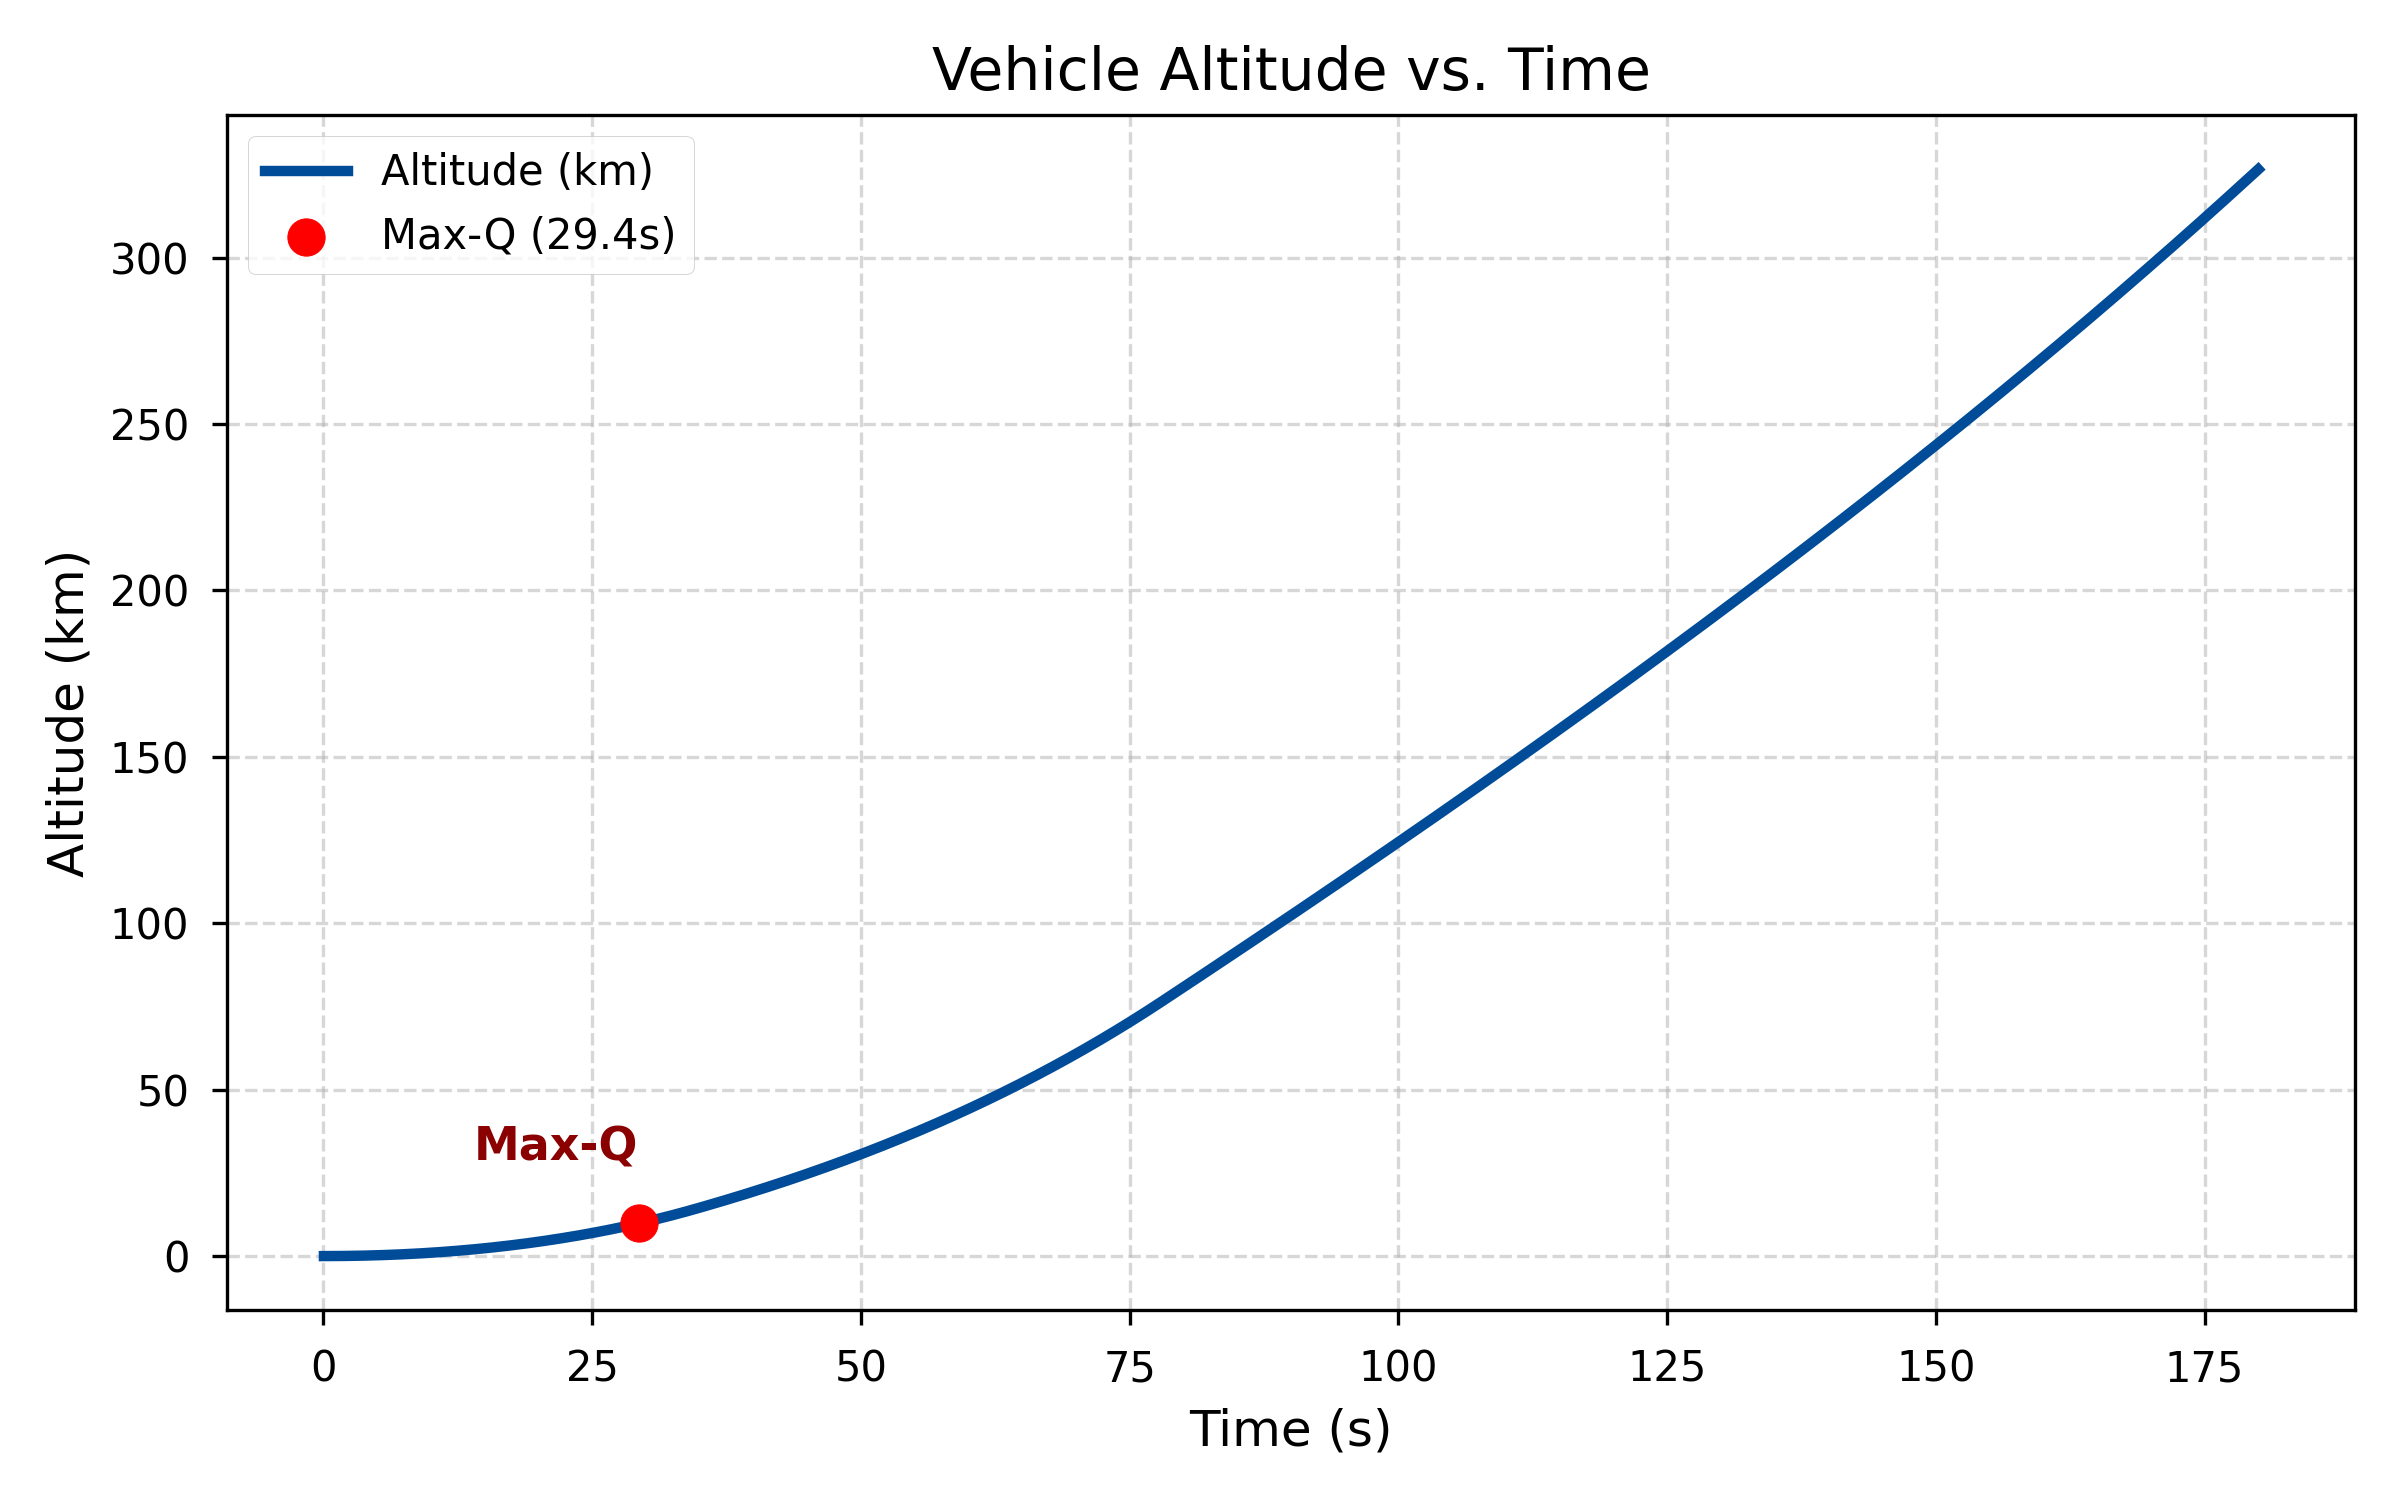
\includegraphics[width=\linewidth]{../figures/fig1_altitude.png}
    \caption{Simulated altitude profile for a PSLV-XL mission to SSO. The point of maximum dynamic pressure (Max-Q) is highlighted.}
    \label{fig:altitude}
\end{figure}

\begin{figure}[htbp]
    \centering
    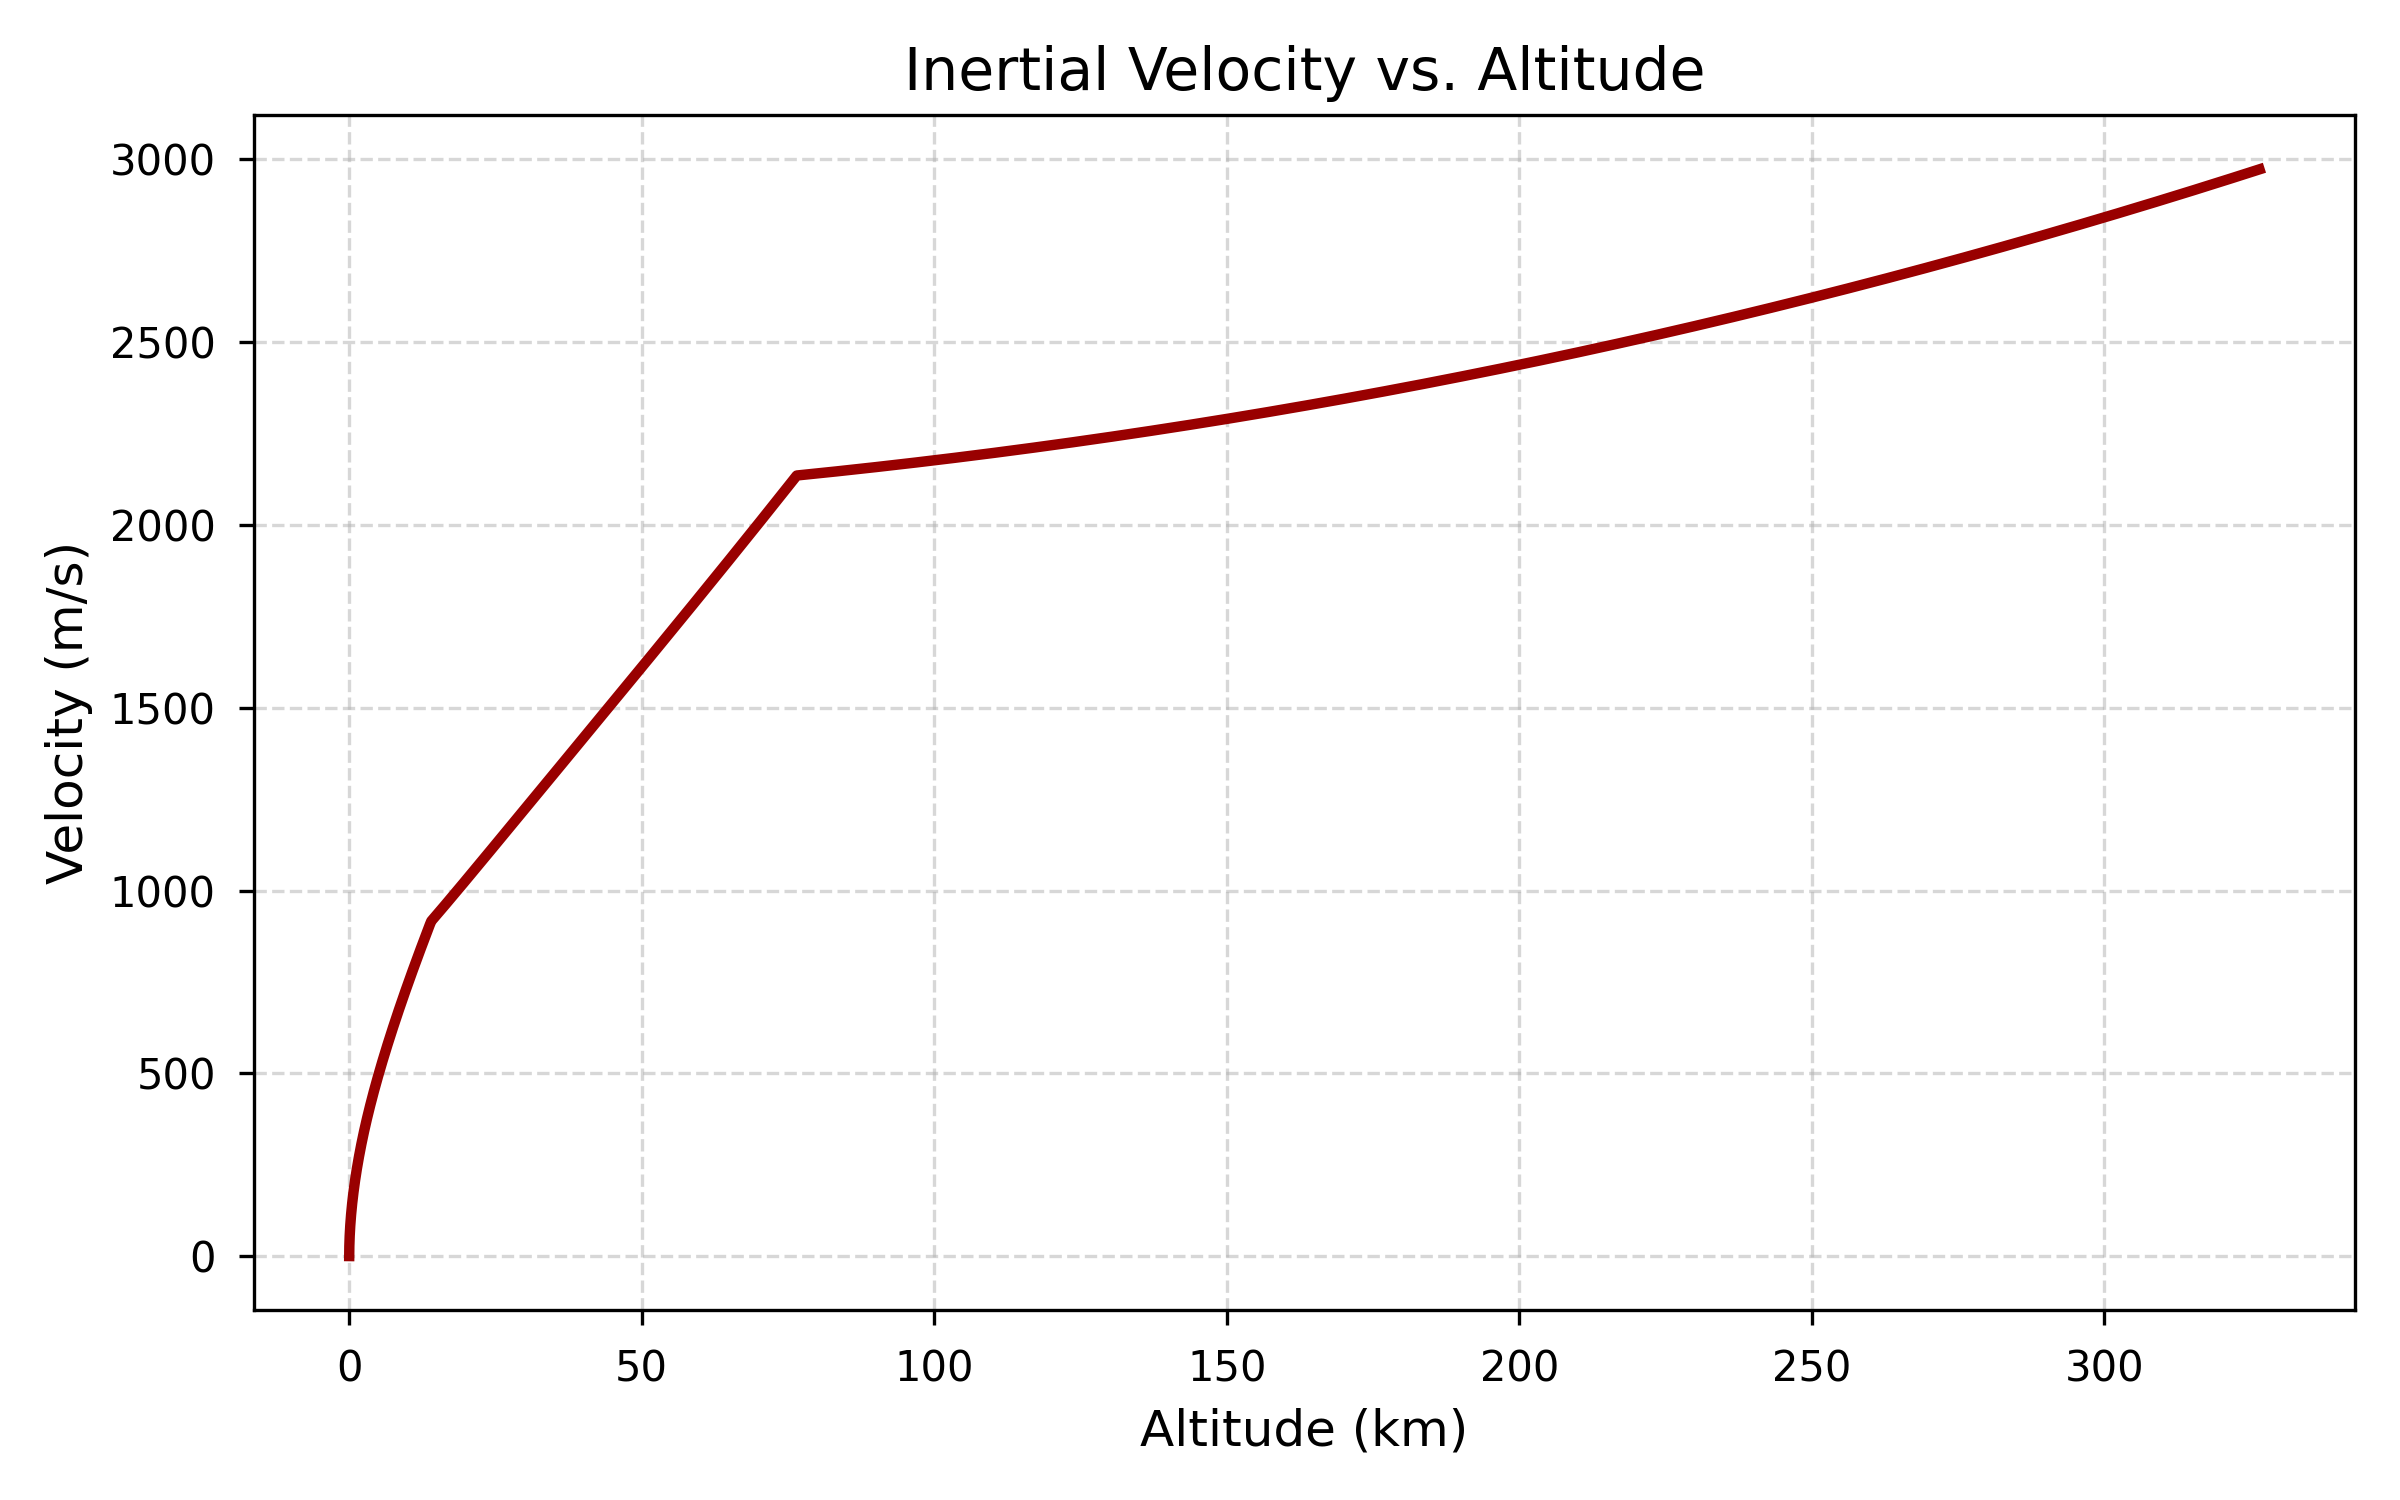
\includegraphics[width=\linewidth]{../figures/fig2_velocity.png}
    \caption{Inertial velocity versus altitude, demonstrating the steep velocity increase post-Max-Q during orbital injection.}
    \label{fig:velocity}
\end{figure}

\begin{figure}[htbp]
    \centering
    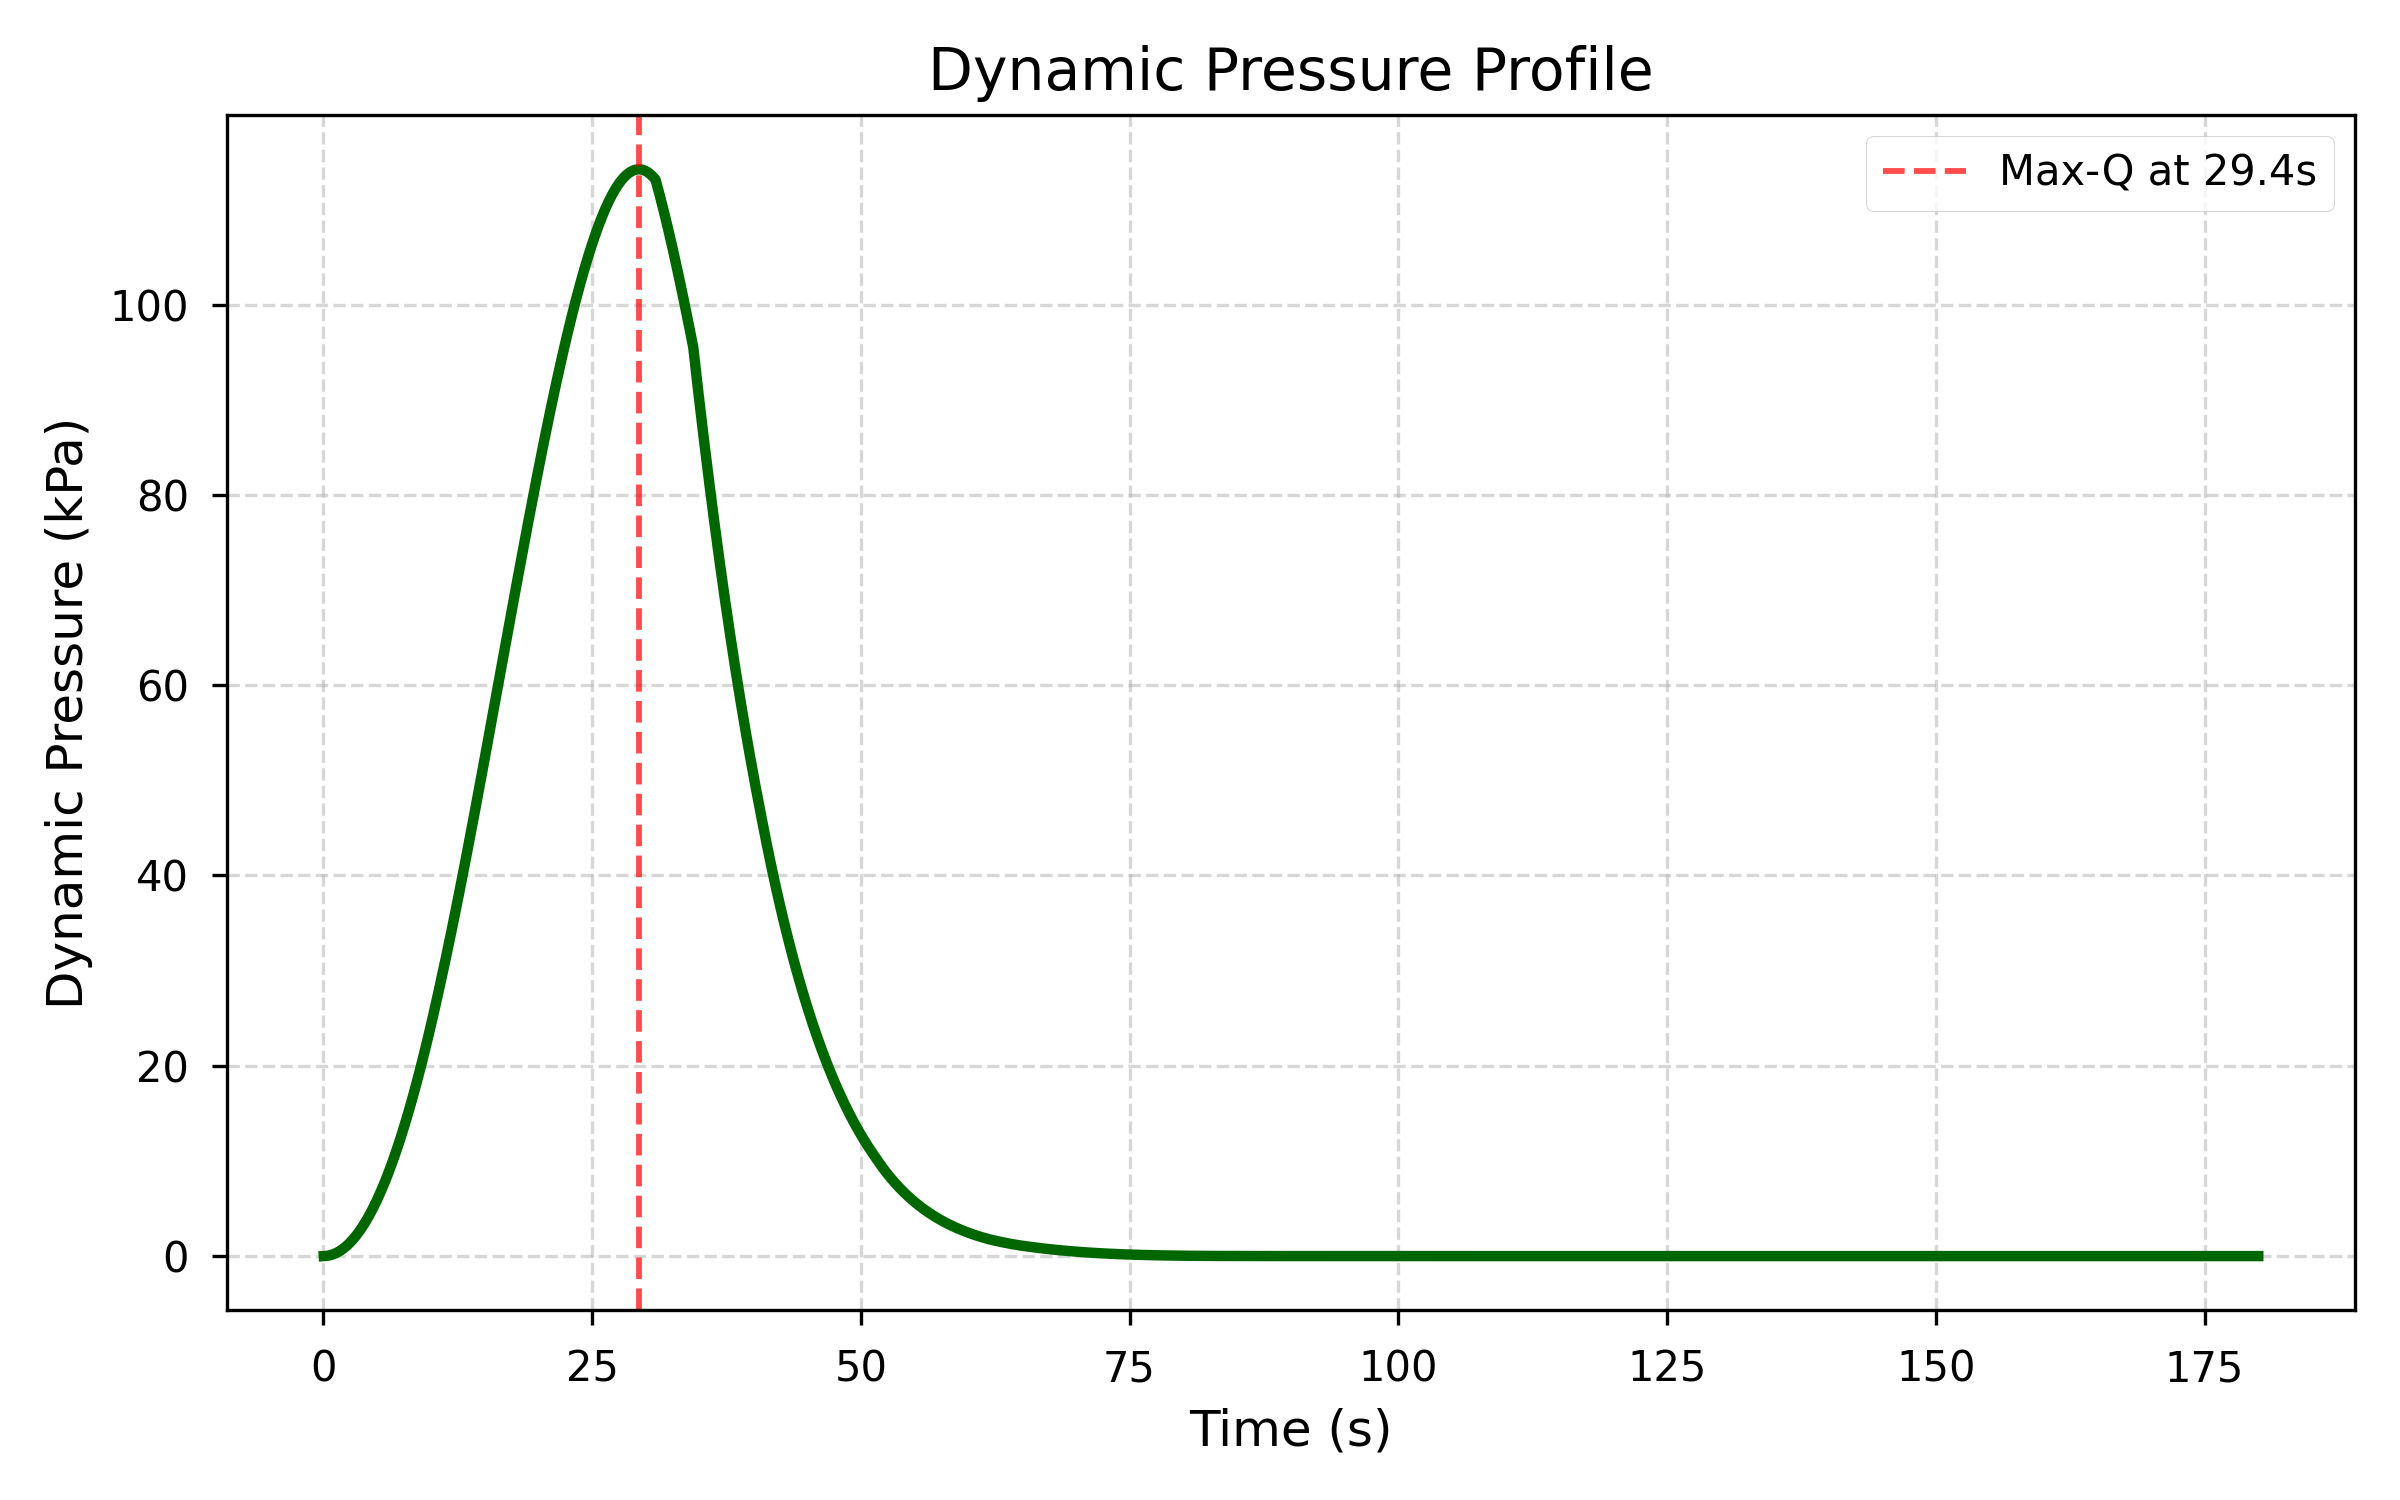
\includegraphics[width=\linewidth]{../figures/fig3_qdyn.png}
    \caption{Dynamic pressure profile over time. The Max-Q constraint is a critical component of the RL reward shaping.}
    \label{fig:maxq}
\end{figure}

RL agent training is currently in progress. Preliminary results indicate that PPO agents converge to viable ascent trajectories within approximately 500,000 environment steps ($\sim$2 hours on a single NVIDIA RTX 3060). Detailed simulation results, RL training curves, and comprehensive performance benchmarks will be presented upon completion of the full system integration.

% ============================================================================
% VIII. CONCLUSION
% ============================================================================
\section{Conclusion}

This paper has presented \textit{Prakshep}, an open-source digital twin and trajectory optimization engine for ISRO launch vehicles. By integrating a high-fidelity C++ 6-DOF physics engine with a sophisticated reinforcement learning framework, \textit{Prakshep} bridges the gap between rigorous aerospace engineering and modern artificial intelligence. The system successfully implements RK4 numerical integration, J2 gravitational perturbations, and Mach-dependent aerodynamics, providing a physically accurate substrate for the RL agents.

The Python-based ML layer demonstrates how dense reward shaping and PPO/SAC algorithms can train autonomous guidance, navigation, and control agents to fly complex, multi-stage vehicles like the PSLV-XL to orbital velocities. Concurrently, the PyTorch LSTM anomaly predictor provides robust, real-time structural integrity forecasting, processing raw telemetry straight from high-efficiency Parquet buffers.

Finally, the full-stack Next.js frontend proves that AAA-quality, real-time visualization can be achieved entirely in the browser using WebGPU and CesiumJS, completely decoupling the physics simulation from the visual presentation. By leveraging a high-performance Zustand WebSocket bridge, the UI provides mission control operators with jitter-free, 60~Hz telemetry rendering inside a state-of-the-art dark-mode aesthetic. 

Future work will pursue validation against real ISRO telemetry data, extension of the physics engine to include multi-body dynamics for spacecraft separation, and implementation of orbital rendezvous scenarios for Gaganyaan mission profiles. \textit{Prakshep} establishes a new standard for zero-cost, open-source aerospace research platforms.

% ============================================================================
% REFERENCES
% ============================================================================
\begin{thebibliography}{20}

\bibitem{butcher2003numerical}
J.~C. Butcher, \textit{Numerical Methods for Ordinary Differential Equations}. Chichester, UK: John Wiley \& Sons, 2003.

\bibitem{vallado2013fundamentals}
D.~A. Vallado, \textit{Fundamentals of Astrodynamics and Applications}, 4th~ed. Hawthorne, CA: Microcosm Press, 2013.

\bibitem{nasa1976atmosphere}
National Oceanic and Atmospheric Administration, National Aeronautics and Space Administration, and United States Air Force, ``U.S. Standard Atmosphere, 1976,'' NASA-TM-X-74335, 1976.

\bibitem{schulman2017proximal}
J.~Schulman, F.~Wolski, P.~Dhariwal, A.~Radford, and O.~Klimov, ``Proximal policy optimization algorithms,'' \textit{arXiv preprint arXiv:1707.06347}, 2017.

\bibitem{haarnoja2018soft}
T.~Haarnoja, A.~Zhou, P.~Abbeel, and S.~Levine, ``Soft actor-critic: Off-policy maximum entropy deep reinforcement learning with a stochastic actor,'' in \textit{Proc. Int. Conf. Mach. Learn. (ICML)}, 2018, pp.~1861--1870.

\bibitem{isro_pslv_manual}
Indian Space Research Organisation, ``PSLV User's Manual,'' ISRO, Bangalore, India, 2019.

\bibitem{isro_gslv_manual}
Indian Space Research Organisation, ``GSLV Mark III User's Manual,'' ISRO, Bangalore, India, 2020.

\bibitem{grieves2002digital}
M.~Grieves, ``Digital twin: Manufacturing excellence through virtual factory replication,'' White Paper, Univ. of Michigan, 2002.

\bibitem{jakob2017pybind11}
W.~Jakob, J.~Rhinelander, and D.~Moldovan, ``pybind11 -- Seamless operability between C++11 and Python,'' 2017. [Online]. Available: \url{https://github.com/pybind/pybind11}

\bibitem{cabello2010threejs}
R.~Cabello \textit{et al.}, ``Three.js -- JavaScript 3D library,'' 2010. [Online]. Available: \url{https://threejs.org}

\bibitem{ramirez2018fastapi}
S.~Ram\'{i}rez, ``FastAPI -- Modern, fast web framework for building APIs with Python,'' 2018. [Online]. Available: \url{https://fastapi.tiangolo.com}

\bibitem{brockman2016openai}
G.~Brockman, V.~Cheung, L.~Pettersson, J.~Schneider, J.~Schulman, J.~Tang, and W.~Zaremba, ``OpenAI Gym,'' \textit{arXiv preprint arXiv:1606.01540}, 2016.

\bibitem{hochreiter1997long}
S.~Hochreiter and J.~Schmidhuber, ``Long short-term memory,'' \textit{Neural Computation}, vol.~9, no.~8, pp.~1735--1780, 1997.

\bibitem{raffin2021stable}
A.~Raffin, A.~Hill, A.~Gleave, A.~Kanervisto, M.~Ernestus, and N.~Dormann, ``Stable-Baselines3: Reliable reinforcement learning implementations,'' \textit{J. Mach. Learn. Res.}, vol.~22, no.~268, pp.~1--8, 2021.

\bibitem{diebel2006representing}
J.~Diebel, ``Representing attitude: Euler angles, unit quaternions, and rotation vectors,'' Stanford University, Tech. Rep., 2006.

\bibitem{brauer1977post}
G.~L. Brauer, D.~E. Cornick, and R.~Stevenson, ``Capabilities and applications of the Program to Optimize Simulated Trajectories (POST),'' NASA CR-2770, 1977.

\bibitem{wie2008spacecraft}
B.~Wie, \textit{Space Vehicle Dynamics and Control}, 2nd~ed. Reston, VA: AIAA, 2008.

\bibitem{sutton2018reinforcement}
R.~S. Sutton and A.~G. Barto, \textit{Reinforcement Learning: An Introduction}, 2nd~ed. Cambridge, MA: MIT Press, 2018.

\end{thebibliography}

\end{document}
